\documentclass[a4paper]{article}

% Packages
\usepackage[left=25mm, top=30mm,]{geometry}
\usepackage{graphicx}
\usepackage{float}
\usepackage{siunitx}
\usepackage{listings}
\usepackage{physics}

% Commands and stuff
\newcommand{\opgave}[1]{\subsection{Opgave #1}}

% Title Page stuff
\title{Practicum Numerieke Modelering en Benadering}
\author{Wim Kunnen \\ Bo Kleynen}
\date{Vrijdag 6 april 2018 }

% Actual document
\begin{document}

\begin{titlepage}
\maketitle
\thispagestyle{empty}
\end{titlepage}

% Table of Contents
\tableofcontents
\thispagestyle{empty}
\cleardoublepage

\pagenumbering{roman}
\setcounter{page}{1}

% List of figures
\listoffigures
\addcontentsline{toc}{section}{\numberline{} Lijst van Figuren}
\cleardoublepage
\pagenumbering{arabic}
\setcounter{page}{1}

% PDE stuff
\section{Partial Differential Equations}\label{sec:PDE}
De eerste opgaven ivm PDE. \\
Vergelijking \ref{eq:PDE} werd opgelost aan de hand van het algoritme in sectie \ref{sec:pde}

\begin{equation}\label{eq:PDE}
	\pdv[2]{u(x,y)}{x} + \pdv[2]{u(x,y)}{y} = f(x,y)
\end{equation}
\opgave{1: Implementatie en controle}\label{sec:oef1}

\opgave{2: Fouten en tijdsduur}\label{sec:oef2}

% Tabel met fouten
\begin{table}[H]
	\centering
	\label{tab:fouten}
	\begin{tabular}{l c r}
		N & Maximale fout & Tijd [seconde] \\ \hline
		8 & \num{1.6118e-04} & 0.002915 \\
		16 & \num{4.5544e-05} & 0.000922 \\		
		32 & \num{1.2136e-05} & 0.000538 \\
		64 & \num{3.1300e-06} & 0.000827 \\
		128 & \num{7.9485e-07} & 0.005202 \\
		256 & \num{2.0027e-07} & 0.013696 \\
		512 & \num{5.0268e-08} & 0.039208 \\
		1024 & \num{1.2605e-08} & 0.231955
	\end{tabular}
	\caption{Tabel met fouten in functie van discretisatie}
\end{table}

\opgave{3: Plot}\label{sec:oef3}
\newpage
% Contour figuur
\begin{figure}[H]
	\begin{center} 
		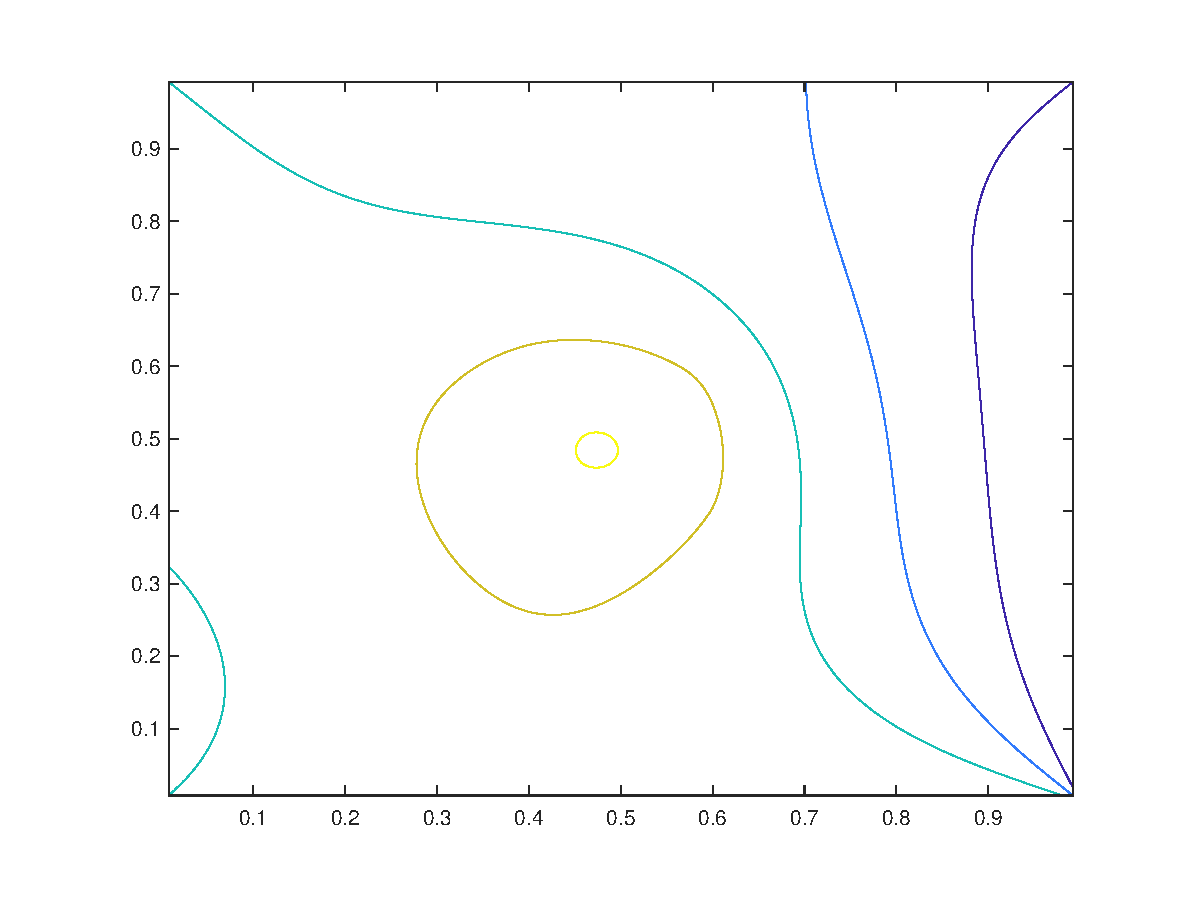
\includegraphics[width=0.7\textwidth]{Contour3.eps}
	\end{center}
	\caption{De contour plot voor Opgave 3.}
	\label{fig:Contour3}
\end{figure}

% Plot
\begin{figure}[H]
	\begin{center} 
		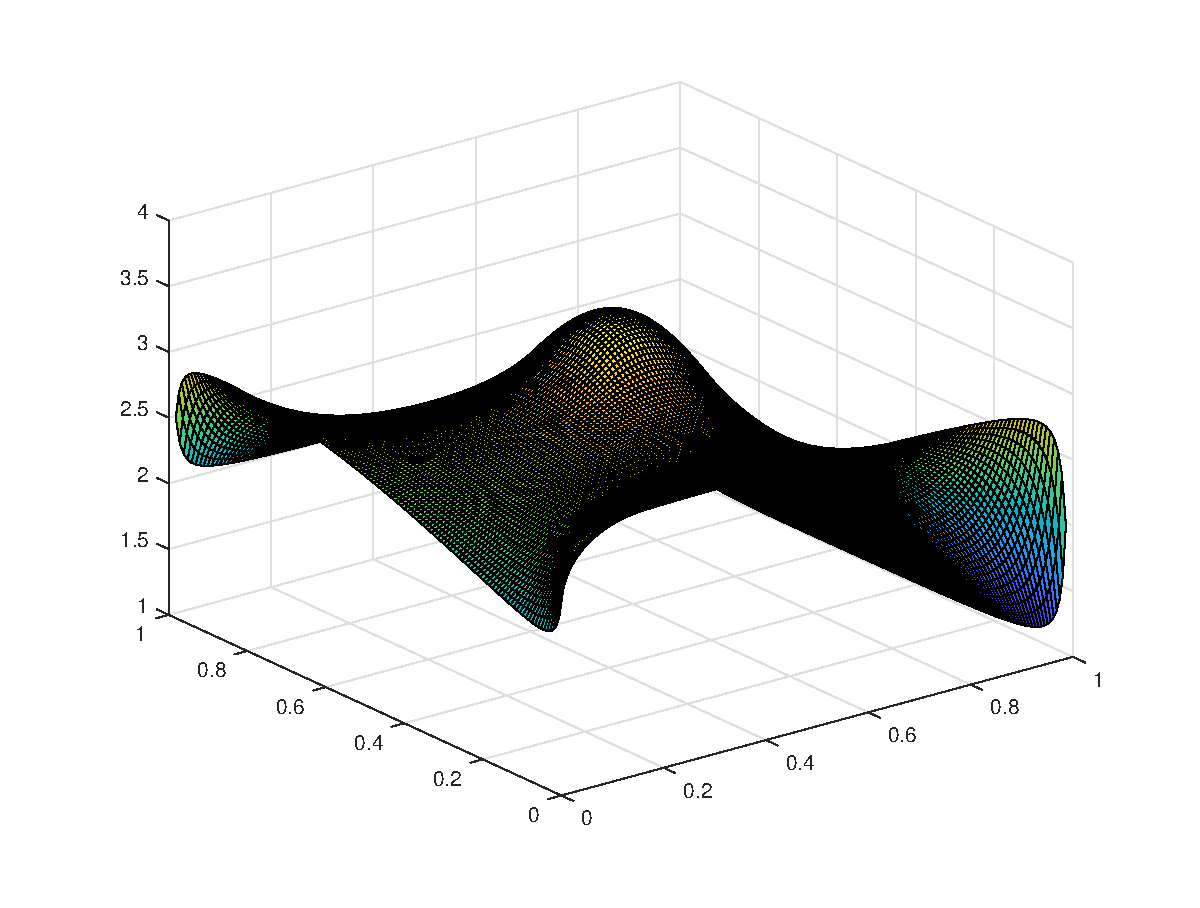
\includegraphics[width=1\textwidth]{Plot3.eps}
	\end{center}
	\caption{De plot voor Opgave 3.}
	\label{fig:Plot3}
\end{figure}
\newpage

% Splines stuff
\section{Splines}\label{sec:splines}

\opgave{4: Implementatie}\label{sec:oef4}

\opgave{5: Illustratie correctheid}\label{sec:oef5}

\opgave{6: Ligging knooppunten}\label{sec:oef6}

\opgave{7: Ruis}\label{sec:oef7}

% Code 'n shit
\newpage
\section{Code}\label{sec:code}

% PDE code
\subsection{PDE Code}\label{sec:generalpde}

\subsubsection{PDE.m}\label{sec:pde}
\lstinputlisting[language=Matlab]{../Matlab/PDE.m}

\subsubsection{Opgave1.m}\label{sec:code1}
\lstinputlisting[language=Matlab]{../Matlab/opgave1.m}

\subsubsection{Opgave2.m}\label{sec:code2}
\lstinputlisting[language=Matlab]{../Matlab/opgave2.m}

\subsubsection{Opgave3.m}\label{sec:code3}
\lstinputlisting[language=Matlab]{../Matlab/opgave3.m}

\newpage
\subsection{Spline Code}\label{sec:generalspline}

\subsubsection{KKB Spline}\label{sec:codekkb}
\lstinputlisting[language=Matlab]{../Matlab/kkb_spline.m}

\subsubsection{deBoor.m}\label{sec:codedb}
\lstinputlisting[language=Matlab]{../Matlab/deBoor.m}

\subsubsection{createM.m}\label{sec:codeM}
\lstinputlisting[language=Matlab]{../Matlab/createM.m}

\subsubsection{Opgave5.m}\label{sec:code5}
\lstinputlisting[language=Matlab]{../Matlab/opgave5.m}

\subsubsection{Opgave6.m}\label{sec:code6}
\lstinputlisting[language=Matlab]{../Matlab/opgave6.m}

\subsubsection{Opgave7.m}\label{sec:code7}
\lstinputlisting[language=Matlab]{../Matlab/opgave7.m}


\end{document}